
% ----------------------------------------------------------
% CAPÍTULO 04 - RESULTADOS
% ----------------------------------------------------------

\chapter{Simulação e Resultados} \label{cha:resultados}

Este capítulo apresenta os resultados da simulação realizada no modelo ORANIG-BR e da microssimulação comportamental para avaliar os efeitos do comércio internacional sobre a desigualdade de renda e pobreza no Brasil. O referido capítulo está dividido em três seções. A primeira descreve a simulação realizada no modelo de equilíbrio geral. A segunda apresenta os resultados do modelo, analisando tanto os efeitos macroeconômicos quanto setoriais, sobre os agentes econômicos, buscando compreender quais foram os grupos beneficiados e prejudicados pela simulação - e a magnitude desse efeito. A terceira e última seção apresenta os resultados do modelo de microssimulação comportamental.



\section{Simulação e mecanismos de transmissão} \label{sec:simulacao}

Propõe-se simular uma política de abertura comercial para avaliar seus efeitos de curto-prazo sobre os indicadores macroeconômicos e setoriais. Essa simulação possibilita mensurar o comportamento das variáveis econômicas frente a uma maior exposição ao comércio internacional, avaliando quais seriam os efeitos de uma política comercial liberalizante.

Por não haver estatísticas mais adequadas para definir a magnitude do choque exógeno desejado neste trabalho, optou-se por realizar uma análise de sensibilidade\footnote{Entende-se por análise de sensibilidade qualquer técnica utilizada para avaliar como variações nas variáveis-chave afetam determinados resultados ou indicadores em um modelo econômico.} -- essencial para situações como esta. Esse tipo de análise é bastante utilizado na literatura econômica, sobretudo em artigos que buscam mensurar impactos de políticas públicas e acordos comerciais \cite{haddad05, domingues08,perobelli17}.

Desse modo, impõe-se aqui uma redução tarifária, através do poder da tarifa, no valor de 10\% sobre todas as \textit{commodities} do modelo. Esse valor foi escolhido após constatar que um aumento na magnitude do choque para além de 10\% não alterava a direção das variáveis macroeconômicos e setoriais. Ademais, ao analisar os resultados microeconômicos, percebe-se que seu comportamento, frente a um progressivo aumento da magnitude do choque, é em formato de U, tendo em 10\% o \textit{breaking point}.

Para fins de facilitar a interpretação dos resultados, optou-se por agregar os setores em seis grandes categorias: 1- Agropecuária; 2- Extrativa; 3- Agroindústria; 4- Indústria; 5- Comércio; e 6- Serviços. A descrição completa dessas categorias, bem como os valores utilizados para realizar o choque da simulação, estão disponíveis, respectivamente, no Apêndice~\ref{ap:a} e~\ref{ap:b} deste trabalho.

A Figura~\ref{fig:mecanismos} exibe os mecanismos de transmissão de uma simulação de redução tarifária no modelo ORANIG-BR. Como citado anteriormente, o comércio internacional pode ser entendido enquanto um choque sobre os preços relativos de uma economia. Aqui, isso ocorre através da tarifa de importação: em geral, os bens de uma economia possuem uma tarifa de importação \textit{ad valorem} que afeta diretamente seu preço. Uma mudança sobre essa tarifa torna por alterar o preço do produto. Essa alteração, por conseguinte, varia os preços relativos do produto no mercado mundial.

O efeito esperado é de queda no preço dos produtos e um consequente aumento das importações, uma vez que se tornou mais barato importar. Isso faz com que o produto internacional se torne mais atrativo frente aos produtos do mercado doméstico, havendo uma pressão interna pelo seu consumo. Além disso, pode-se esperar mudança nos retornos dos fatores produtivos dado os novos preços relativos -- como visto no modelo H-O. Como consequência, impõe-se algum nível de reestruturação produtiva a partir dos novos preços e retornos dos fatores produtivos, ajustando-se de acordo com os incentivos.

Sobre as firmas, espera-se um ganho de produtividade das empresas que sejam beneficiadas pela redução tarifária, aumentando sua competitividade no cenário doméstico. Isso fará com que haja uma variação positiva na produção e negativa no índice de preços da economia. Esse novo cenário afeta a renda real de todos os agentes econômicos, beneficiando ou prejudicando os grupos de acordo com a distribuição funcional da renda.

Também é possível esperar um efeito substituição como consequência de uma redução tarifária. Isso pode ocorrer por conta da variação dos preços relativos, que pode tornar mais atrativo importar determinados insumos que consumir sua opção doméstica. Dado esse efeito, espera-se uma variação no produto final, produzido domesticamente, já que houve uma variação no custo de produção. Como último estágio, o efeito substituição gera uma variação na intensidade do comércio internacional, dado a mudança na composição de bens domésticos e importados para produção dos bens nacionais.

Vale a pena ressaltar que também é esperado alguns efeitos \textit{feedback} sempre que haja alteração dos preços e do índice de preços da economia -- que são captados pelo modelo de equilíbrio geral, gerando novas rodadas de efeitos macroeconômicos e setoriais.


\begin{figure}[H]
	\centering
	\caption{Mecanismos de transmissão de uma redução tarifária no modelo ORANIG-BR} \label{fig:mecanismos}
	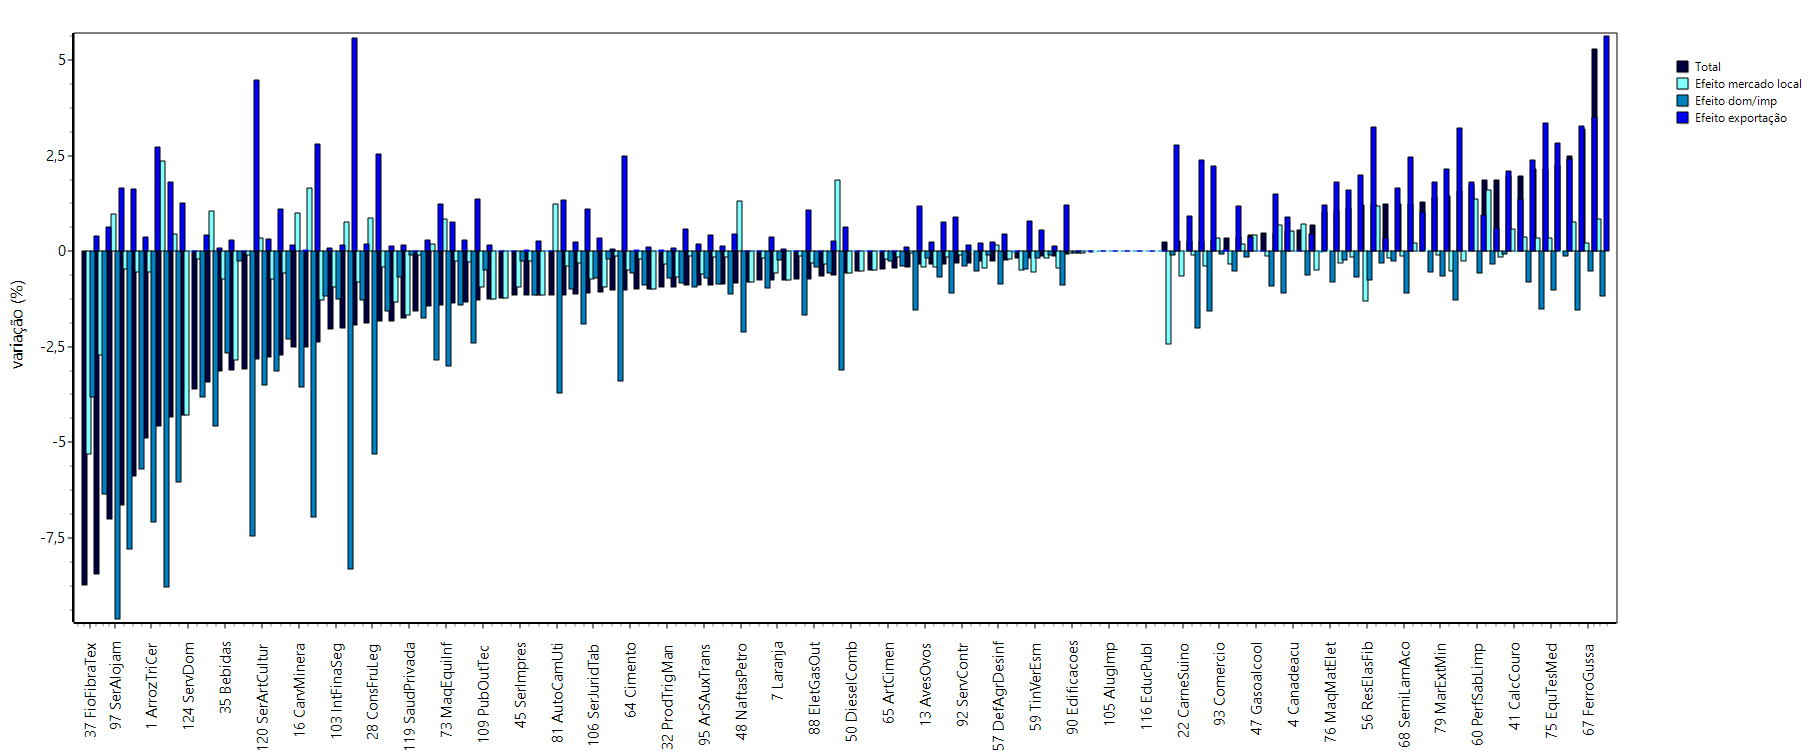
\includegraphics[width=\textwidth]{Imagens/007.ai}
	\footnotesize
	Fonte: elaboração própria (2024) a partir de \textcite{vinicius18}.
\end{figure}



\section{Resultados do modelo ORANIG-BR} \label{sec:resultados}

A Tabela~\ref{tab:result} apresenta os resultados macroeconômicos do modelo. Percebe-se que a redução tarifária afetou negativamente todos os indicadores de preços, com destaque para o índice preço do consumidor (-0,1156\%), do investimento (-0,1999) e das importações -- que registrou a maior queda: -0,4623\%. A queda conjunta dos preços das exportações e importações incentivaram o aumento da corrente de comércio, sendo liderado pela variação positiva do volume importado (0,1909\%). Esse aumento, largamente composto por insumos voltados à atividade industrial, como apresentado na Tabela~\ref{tab:import}, tornou por baratear os custos da produção nacional, resultando em um aumento do emprego real (0,0358\%) e do PIB real (0,0256\%) -- ainda que em valores diminutos. A expansão do volume importado também favoreceu as famílias, que experimentaram um aumendo do consumo real no valor de 0,0555\%.

O deflator do PIB, entendido enquanto um índice de preços implícito que mede a evolução média de preços numa economia, reduziu em 0,1416\%. Esse resultado, em conjunto com o aumento do PIB e emprego real, permite afirmar que a redução tarifária trouxe efeitos positivos sobre os indicadores macroeconômicos, uma vez que se experimentou aumento da atividade econômica e redução dos preços da economia em geral. Entretanto, a variação negativa dos termos de troca (-0,0973), ainda que tímida, aponta que esse cenário não é sustentável no longo-prazo, já que as exportações estão perdendo sua capacidade de financiar as importações. 


\begin{table}[h]
	\centering
	\small
	\begin{threeparttable}
		\caption{Efeitos macroeconômicos de curto-prazo da redução tarifária} \label{tab:result}
		\begin{tabular}{m{11cm}c}
			\hline
			\multirow{2}{*}{\textbf{Indicadores}} & \multirow{2}{*}{\textbf{Var. (\%)}} \\
			 &  \\ \hline
			\textbf{Preços} &  \\
			\hspace{0.2cm} Índice de preços do consumidor & -0,1156 \\
			\hspace{0.2cm} Índice de preços do investimento & -0,1999 \\
			\hspace{0.2cm} Índice de preços do governo & -0,1103 \\
			\hspace{0.2cm} Índice de preços das exportações & -0,0973 \\
			\hspace{0.2cm} Índice de preços das importações & -0,4623 \\
			\hspace{0.2cm} Índice de preços do PIB & -0,1416 \\
			\hspace{0.2cm} Termos de troca & -0,0973 \\
			\hspace{0.2cm} Custos dos fatores primários & -0,0617 \\
			\hspace{0.2cm} Salário nominal & -0,1156 \\
			\hspace{0.2cm} Desvalorização real & 0,1418 \\ \hline
			\textbf{Volume} &  \\
			\hspace{0.2cm} Consumo real das famílias & 0,0555 \\
			\hspace{0.2cm} Volume exportado & 0,1009 \\
			\hspace{0.2cm} Volume importado & 0,1909 \\
			\hspace{0.2cm} PIB real & 0,0256 \\
			\hspace{0.2cm} Emprego real & 0,0358 \\ \hline
		\end{tabular}
	\begin{tablenotes}
		\footnotesize
		\item Fonte: elaboração própria (2024) com base nas simulações feitas no ORANIG-BR.
	\end{tablenotes}
	\end{threeparttable}
\end{table}

A Tabela~\ref{tab:ativ} apresenta os resultados setoriais da redução tarifária sobre o nível de atividade econômica e emprego, selecionando os dez setores produtivos com as maiores e menores variações percentuais no nível de atividade. As correspondências dos setores estão disponíveis no Apêndice~\ref{ap:a}.

Os setores mais beneficiados foram aqueles que utilizam os insumos importados que tiveram as maiores reduções em seus preços de importações. Foi o caso do setor de Fabricação de calçados e de artefatos de couro (C15) que experimentou a maior variação no nível de atividade econômica (0,1849\%) e emprego (0,2483\%). Como apresentado na Tabela~\ref{tab:import}, a \textit{commodity} Tecido (C38) foi a que registrou a maior variação negativa em seu preço de importação e, por conseguinte, maior variação positiva em seu volume importado. Essa \textit{commodity} representa, sozinha, quase 20\% dos produtos importados pelo setor de Fabricação de calçados. Desse modo, a redução tarifária funcionou como um corte de custos de produção, permitindo expandir seu nível de produção e emprego.

É possível notar que as maiores variações positivas não se concentraram em nenhum dos setores agregados: quatro desses seis grandes setores estão entre aqueles com maior expansão do nível de atividade econômica. Entretanto, as maiores variações negativas estão concentradas no setor industrial, com destaque para Fabricação de produtos têxteis (C13) que registrou a maior retração de sua atividade econômica (-0,6101\%) e emprego (-0,7916\%). Essa concentração no setor industrial é explicada pela perda de competitividade desses setores frente a uma maior abertura comercial. Ou seja, a redução tarifária reduziu o \textit{market share} desses setores na economia doméstica. A Tabela~\ref{tab:fandecomp} apresenta os dados que corroboram essa afirmação, sendo discutida em detalhes mais abaixo.


\begin{table}[h]
	\centering
	\small
	\begin{threeparttable}
		\caption{Efeitos de curto-prazo da redução tarifária sobre o nível de atividade e emprego (var. \%)}\label{tab:ativ}
		\begin{tabular}{m{2cm} >{\centering\arraybackslash}m{4cm} >{\centering\arraybackslash}m{4cm} >{\centering\arraybackslash}m{4cm} >{\centering\arraybackslash}m{4cm}}
			\hline
			\multirow{2}{*}{\textbf{Setores}} & \multirow{2}{*}{\textbf{Setores agregados}} & \multicolumn{2}{c}{\textbf{Indicadores}} \\ \cline{3-4} &  & \textbf{Nível de atividade} & \textbf{Emprego} \\ \hline
			C15 & Indústria     & 0,1849  & 0,2483 \\
			C35 & Indústria     & 0,1148  & 0,1379 \\
			C44 & Serviços      & 0,0809  & 0,1079 \\
			C37 & Serviços      & 0,0802  & 0,1472 \\
			C07 & Extrativa     & 0,0743  & 0,1413 \\
			C65 & Serviços      & 0,0661  & 0,0661 \\
			C60 & Serviços      & 0,0636  & 0,0690 \\
			C23 & Indústria     & 0,0618  & 0,0891 \\
			C62 & Serviços      & 0,0531  & 0,1027 \\
			C12 & Agroindústria & 0,0489  & 0,1476 \\ \hline
			C13 & Indústria     & -0,6101 & -0,7916 \\
			C14 & Indústria     & -0,1955 & -0,2686 \\
			C25 & Indústria     & -0,1342 & -0,1652 \\
			C36 & Indústria     & -0,1041 & -0,1985 \\
			C29 & Indústria     & -0,0368 & -0,0543 \\
			C33 & Indústria     & -0,0279 & -0,0298 \\
			C26 & Indústria     & -0,0251 & -0,0339 \\
			C16 & Indústria     & -0,0193 & -0,0314 \\
			C21 & Indústria     & -0,0099 & -0,0215 \\
			C27 & Indústria     & -0,0085 & -0,0149 \\ \hline
			\end{tabular}
		\begin{tablenotes}
			\footnotesize
			\item Fonte: elaboração própria (2024) com base nas simulações feitas no ORANIG-BR.
		\end{tablenotes}
		\end{threeparttable}
\end{table}

A Tabela~\ref{tab:fandecomp} apresenta a decomposição dos efeitos de curto-prazo da redução tarifária em quatro categorias: 1- Mercado Local; 2- Substituição; 3- Exportação; e 4- Total. A primeira deve ser entendida enquanto o nível de produção esperado dado uma mudança na demanda interna do produto, independentemente da fonte -- se doméstico ou importado. A segunda pode ser interpretada como o valor pelo qual a produção dos bens nacionais varia devido a uma mudança relativa de preços que favoreça a substituição de importações. A terceira mostra a contribuição da variação das exportações para a variação da produção nacional. A quarta e última coluna é a soma dos valores das três outras categorias.

O efeito Mercado Local foi o responsável pelas maiores variações positivas do efeito Total. Dentre essas, destacam-se as \textit{commodities} mais relacionadas com a Indústria: Calçados e artefatos de couro (C41), Aeronaves, embarcações e outros equipamentos de transporte (C84) e Eletrodomésticos (C77). Isso significa que a produção desses bens teria que ter aumentado na magnitude do efeito Mercado Local para poder ter atendido a pressão sobre a demanda realizada pelo corte tarifário.

Por outro lado, o efeito Substituição foi dominante nas maiores variações negativas do efeito Total. Isso significa que esses produtos perderam competitividade no mercado doméstico frente a uma maior exposição ao mercado internacional. Dentre esses, pode-se destacar as \textit{commodities} Tecido (C38), Fios e fibras têxteis beneficiadas (C37) e Art. têxteis de uso doméstico e outros têxteis (C39).

Desse modo, pode-se afirmar que a indústria foi o setor agregado mais afetado pela redução tarifária, havendo uma parcela de si por ela beneficiada -- como, por exemplo, os setores voltados para a fabricação de couro e calçado -- e outra parcela por ela prejudicada -- neste caso, os setores voltados para a fabricação têxtil. Como expõe a Tabela~\ref{tab:ativ}, os setores relacionados com Serviços, Extrativa e Agroindústria também foram beneficiados pela abertura comercial, entretanto, gozando de um ganho mais diminuto.


\begin{table}[H]
	\centering
	\small
	\begin{threeparttable}
		\caption{Decomposição dos efeitos de curto-prazo da redução tarifária (var. \%)} \label{tab:fandecomp}
		\begin{tabular}{lccccc}
		\hline
		\multirow{2}{*}{\textit{\textbf{Commodities}}} &
		\multicolumn{1}{c}{\multirow{2}{*}{\textbf{Setores agregados}}} &
		\multicolumn{4}{c}{\textbf{Efeitos}} \\ \cline{3-6} 
		&
		\multicolumn{1}{c}{} &
		\multicolumn{1}{c}{\textbf{Mercado local}} &
		\multicolumn{1}{c}{\textbf{Substituição}} &
		\multicolumn{1}{c}{\textbf{Exportação}} &
		\multicolumn{1}{c}{\textbf{Total}} \\ \hline
		C41  &	Indústria	  &	 0,1275	&  0,0001 &	0,0514	&  0,1790	\\	
        C84  &	Indústria	  &	 0,0323	&  -0,006 &	0,0846	&  0,1109	\\	
		C77  &	Indústria	  &	 0,0974	&  -0,024 &	0,0053	&  0,0788	\\	
		C97  &	Serviços	  &	 0,0189	&  0,0354 &	0,0240	&  0,0783	\\	
		C72  &	Indústria	  &	 0,0326	&  0,0059 &	0,0388	&  0,0774	\\	
		C20  &	Extrativa	  &	 0,0173	&  0,0057 &	0,0461	&  0,0691	\\	
		C124 &	Serviços	  &	 0,0661	&  0      &	0	    &  0,0661	\\	
		C79  &	Indústria	  &	 0,0093	& -0,0061 &	0,0610	&  0,0643	\\	
		C87  & 	Serviços	  &	 0,0149	&  0,0424 &	0,0068	&  0,0641	\\	
		C117 & 	Serviços	  &	 0,0608	&  0,0009 &	0,0001	&  0,0618	\\	\hline
		C38  & 	Indústria	  &	-0,1082	& -0,6980 &	0,0412	& -0,7650	\\	
		C37  &	Indústria	  &	-0,3986	& -0,2799 &	0,0189	& -0,6596	\\	
		C39  & 	Indústria	  &	-0,0042	& -0,4037 &	0,0054	& -0,4025	\\	
		C86  &	Indústria	  &	 0,0897	& -0,3485 &	0,0502	& -0,2086	\\	
		C40  &	Indústria	  &	 0,2318	& -0,4374 &	0,0057	& -0,1999	\\	
		C62  &	Indústria	  &	 0,0319	& -0,3109 &	0,1234	& -0,1556	\\	
		C63  &	Indústria	  &	-0,0032	& -0,1508 &	0,0261	& -0,1279	\\	
		C03  &	Agropecuária  &	-0,1934	& -0,0012 &	0,1318	& -0,0627	\\	
		C56  &	Indústria	  &	-0,0772	& -0,0322 &	0,0521	& -0,0574	\\	
		C24  &	Agroindústria &	 0,0705	& -0,1505 &	0,0276	& -0,0524	\\	\hline

		\end{tabular}
	\begin{tablenotes}
		\footnotesize
		\item Fonte: elaboração própria (2024) com base nas simulações feitas no ORANIG-BR.
	\end{tablenotes}
	\end{threeparttable}
\end{table}


A Tabela~\ref{tab:import} exibe os efeitos de curto-prazo da redução tarifária sobre o volume e preço das importações por \textit{commodity}. A maior exposição ao mercado internacional aumentou a demanda pelos produtos dos setores da Indústria, Agroindústria e Agropecuária. Como citado anteriormente, a expansão nas importações desses produtos, em especial Tecido (C38), Artigos do vestuário e acessórios (C40) e Art. têxteis de uso doméstico e outros têxteis (C39), é resultado da redução dos custos de produção proporcionada pelo corte tarifário, que tornou por baixar o preço de importação desses bens. Os menores preços permitiram uma expansão no nível de atividade e emprego dos setores que tem esses bens como insumos.

A segunda metade da Tabela apresenta as \textit{commodities} com as maiores variações negativas de volume importado. Isso se deu por conta que esses bens já não contavam com nenhuma barreira tarifária, logo, seus preços de importações não foram afetados pelo corte tarifário. O volume importado tornou por reduzir por conta da mudança dos preços relativos que pressionaram a demanda por importações de outros produtos, esses sim, afetados pelo corte tarifário.


\begin{table}[h]
	\centering
	\small
	\begin{threeparttable}
		\caption{Efeitos de curto-prazo da redução tarifária sobre as importações (var. \%)} \label{tab:import}
		\begin{tabular}{m{3cm} >{\centering\arraybackslash}m{3cm} >{\centering\arraybackslash}m{3cm} >{\centering\arraybackslash}m{3cm}}
			\hline
			\multirow{2}{*}{\textit{\textbf{Commodities}}} & \multirow{2}{*}{\textbf{Setores agregados}} & \multicolumn{2}{c}{\textbf{Importações}} \\ \cline{3-4} 
			      &               & \textbf{Volume} & \textbf{Preço} \\ \hline
			 C38  & Indústria     &  2,7413         & -2,6082 \\
			 C40  & Indústria     &  2,6257         & -2,4429 \\
			 C39  & Indústria     &  1,9852         & -1,6339 \\
			 C27  & Agroindústria &  1,4747         & -0,5882 \\
			 C42  & Indústria     &  1,4279         & -0,8667 \\
			 C6   & Agropecuária  &  1,2962         & -0,9169 \\
			 C34  & Agroindústria &  1,2562         & -1,1298 \\
			 C63  & Indústria     &  1,2292         & -1,1688 \\
			 C37  & Agroindústria &  1,2211         & -1,7473 \\ \hline
			 C90  & Serviços      & -0,1760         & 0       \\
			 C87  & Serviços      & -0,1648         & 0       \\
			 C92  & Serviços      & -0,1412         & 0       \\
			 C102 & Serviços      & -0,0953         & 0       \\
			 C96  & Comércio      & -0,0925         & 0       \\
			 C111 & Serviços      & -0,0891         & 0       \\
			 C112 & Serviços      & -0,0868         & 0       \\
			 C23  & Extrativa     & -0,0798         & 0       \\
			 C94  & Serviços      & -0,0618         & 0       \\ \hline
			\end{tabular}
		\begin{tablenotes}
			\footnotesize
			\item Fonte: elaboração própria (2024) com base nas simulações feitas no ORANIG-BR.
		\end{tablenotes}
		\end{threeparttable}
\end{table}

A literatura econômica afirma que o comércio internacional gera ganhadores e perdedores. Os resultados do modelo ORANIG-BR indicam que uma redução tarifária beneficiaria os setores da Agroindústria, Agropecuária e uma parte da Indústria -- mais relacionada com produção de tecidos e calçados. Por outro lado, haveria perda de \textit{market share} de uma outra parcela industrial brasileira, mais relacionada com a produção têxtil, reduzindo, por conseguinte, seu nível de atividade econômica. Entretanto, os indicadores macroeconômicos sugerem que os ganhos do primeiro grupo foram capazes de superar as perdas do segundo grupo, levando a uma redução dos preços da economia e um aumento do PIB real, emprego agregado e consumo das famílias.

Esse resultado levanta discussões na literatura econômica relacionados com a temática de reestruturação da produção e da pauta exportadora brasileira, bem como a temática da desindustrialização e reprimarização da pauta exportadora. Entretanto, os dados são insuficientes para realizar qualquer inferência sobre esse bloco temático.



\section{Resultados da microssimulação comportamental} \label{sec:microssimulacao}

Os resultados do modelo de geração da renda familiar estão expostos na Tabela~\ref{tab:result_microssimulacao}. Como descrito na subseção~\ref{subsec:integracao}, após estimar o cenário \textit{benchmarking} da microssimulação, usa-se os parâmetros de emprego e salários, obtidos no modelo ORANIG-BR, para estimar uma nova rodada de microssimulação, aqui chamada de cenário integração. Os índices de Gini e FGT são calculados em cima desses dois cenários, observando a variação desses indicadores entre o benchmarking e integração -- que expressa os efeitos do choque exógeno sobre a desigualdade de renda e pobreza.

Os coeficientes da Correção de Heckman e da escolha ocupacional, bem como os resultados do cenário \textit{benchmarking} e os parâmetros de variação de salário e emprego estão disponíveis no Apêndice~\ref{ap:b}.

\begin{table}[h]
	\centering
	\small
	\begin{adjustwidth}{-1.5cm}{}
	\begin{threeparttable}
		\caption{Microssimulação dos efeitos da redução tarifária sobre desigualdade de renda e pobreza por qualificação} \label{tab:result_microssimulacao}
	\begin{tabular}{lcccccc}
	\hline
	\multirow{4}{*}{\textbf{}} & \multicolumn{2}{c}{\multirow{2}{*}{\textbf{Não qualificado}}} & \multicolumn{2}{c}{\multirow{2}{*}{\textbf{Semi-qualificado}}} & \multicolumn{2}{c}{\multirow{2}{*}{\textbf{Qualificado}}} \\
	 & \multicolumn{2}{c}{} & \multicolumn{2}{c}{} & \multicolumn{2}{c}{} \\ \cline{2-7} 
	 & \multirow{2}{*}{\textbf{Simulado}} & \multirow{2}{*}{\textbf{Variação (\%)}} & \multirow{2}{*}{\textbf{Simulado}} & \multirow{2}{*}{\textbf{Variação (\%)}} & \multirow{2}{*}{\textbf{Simulado}} & \multirow{2}{*}{\textbf{Variação (\%)}} \\
	 &  &  &  &  &  &  \\ \hline
	\textbf{Pobreza$^{\dag}$}    		          &       &        &       &        &       &        \\[3pt]
	\hspace{0.2cm} $\text{FGT}_0$   		  	  & 39,16 & 0,081  & 19,50 & 0,102  & 8,18  & 0,155  \\[3pt]
	\hspace{0.2cm} $\text{FGT}_1$   	  		  & 17,96 & 0,092  & 8,41  & 0,124  & 4,75  & 0,066  \\[3pt]
	\hspace{0.2cm} $\text{FGT}_2$   	   		  & 11,15 & 0,078  & 5,39  & 0,086  & 3,70  & 0,044  \\[3pt] \hline
	\textbf{Extrema pobreza$^{\ddagger}$} &       &        &       &        &       &                \\[3pt]
	\hspace{0.2cm} $\text{FGT}_0$   			  & 10,61 & 0,101  & 5,21  & 0,021  & 3,93  & --     \\[3pt]
	\hspace{0.2cm} $\text{FGT}_1$   		  	  & 5,02  & 0,031  & 3,00  & 0,022  & 2,74  & 0,023  \\[3pt]
	\hspace{0.2cm} $\text{FGT}_2$       		  & 3,21  & 0,022  & 2,21  & 0,019  & 2,31  & 0,019  \\[3pt] \hline
	\textbf{Desigualdade de renda}                &       &        &       &        &       &        \\[3pt]
	\hspace{0.2cm} Gini                           & 0,457 & -0,022 & 0,442 & -0,012 & 0,487 & -0,011 \\[3pt] \hline
	\end{tabular}
	\begin{tablenotes}
		\footnotesize
		\item Fonte: elaboração própria (2024) com base nos dados da PNAD 2015.
		\item \textit{Nota:}
		\item \hspace{0.2cm} $^{\dag}$     Indivíduos com renda familiar per capita abaixo de R\$367,02.
		\item \hspace{0.2cm} $^{\ddagger}$ Indivíduos com renda familiar per capita abaixo de R\$126,79.
	\end{tablenotes}
	\end{threeparttable}
	\end{adjustwidth}
\end{table}

Os resultados apontam que o potencial da abertura comercial para afetar a desigualdade de renda e pobreza é um tanto limitado, uma vez que seus índices variaram muito pouco. Mesmo assim, observou-se uma redução na desigualdade de renda para os três níveis de qualificação, ao passo em que se experimentou um aumento generalizado nos níveis de pobreza e de pobreza extrema.

Olhando os indicadores de pobreza, as maiores variações foram na proporção de pobres para os semi-qualificados (0,102\%) e qualificados (0,155\%) e na intensidade da pobreza para os semi-qualificados (0,124\%). Ou seja, a redução tarifária realizou, para esses grupos, um aumento no quantitativo de pobres e os distanciou da linha de pobreza. Não houve variação relevante na severidade da pobreza.

Sobre a extrema pobreza, a única variação relevante se deu na proporção de pobres para os não-qualificados (0,101\%). Todos os outros resultados foram bem limitados, com variações na segunda casa decimal. Isso chama atenção, particularmente, mostrando que, para níveis extremos de pobreza, o comércio internacional é praticamente nulo.

O mesmo cenário se repete quando se analisa a desigualdade de renda. Para os três grupos observados, praticamente nada se alterou: todas as variações foram apenas na segunda casa decimal (-0,022\%, -,0012\% e -0,011\% respectivamente). Entretanto, é interessante destacar a direção dos efeitos. Em contraste com o comportamento da pobreza e extrema pobreza, a microssimulação registrou uma redução da desigualdade para os três grupos -- ainda que numa diminuta magnitude.

Desse modo, pode-se afirmar que, de acordo com os resultados da microssimulação, uma redução tarifária no montante de 10\% levou ao aumento da pobreza absoluta e extrema para as três categorias de qualificação, ao passo em que se observou uma redução dos níveis de desigualdade. Para além disso, a microssimulação também constatou que o comércio internacional tem um potencial limitado para afetar esses indicadores de maneira expressiva, sobretudo para os extremamente pobres.

Existem diversas evidências na literatura econômica que convergem para os resultados aqui encontrados. Tanto sobre a diminuta influência do comércio internacional \cite{carneiro06} quanto sobre os resultados divergentes entre desigualdade de renda e pobreza \cite{borrazetal12}.

Por fim, várias razões podem explicar o comportamento dos indicadores de desigualdade de renda e pobreza encontrados. Sobre a diminuta influência, uma das razões pode ser que as barreiras tarifárias já não sejam altas o suficiente para que uma nova redução traga efeitos expressivos. Um possível teste para essa hipótese seria simular um aumento das barreiras tarifárias e observar seus efeitos sobre a desigualdade de renda e pobreza.

Uma possível razão que explique o generalizado aumento da pobreza absoluta e extrema, ainda que parco, pode estar relacionado a estrutura produtiva brasileira e seu perfil de pauta exportadora. Como vimos anteriormente, a redução tarifária afetou proporcionalmente os setores da Agroindústria, pouco intensiva em trabalho, e prejudicando os setores industriais de produção têxtil, comparativamente mais intensivos em trabalho. Essa distribuição, somada a uma redução do salário nominal em 0,11\%, pode explicar o aumento da pobreza. Entretanto, não é possível testar quaisquer dessas suposições com a estratégia empírica aqui utilizada.


